\section{RAS\_\-perfect\_\-t Class Reference}
\label{classRAS__perfect__t}\index{RAS\_\-perfect\_\-t@{RAS\_\-perfect\_\-t}}
Inheritance diagram for RAS\_\-perfect\_\-t:\nopagebreak
\begin{figure}[H]
\begin{center}
\leavevmode
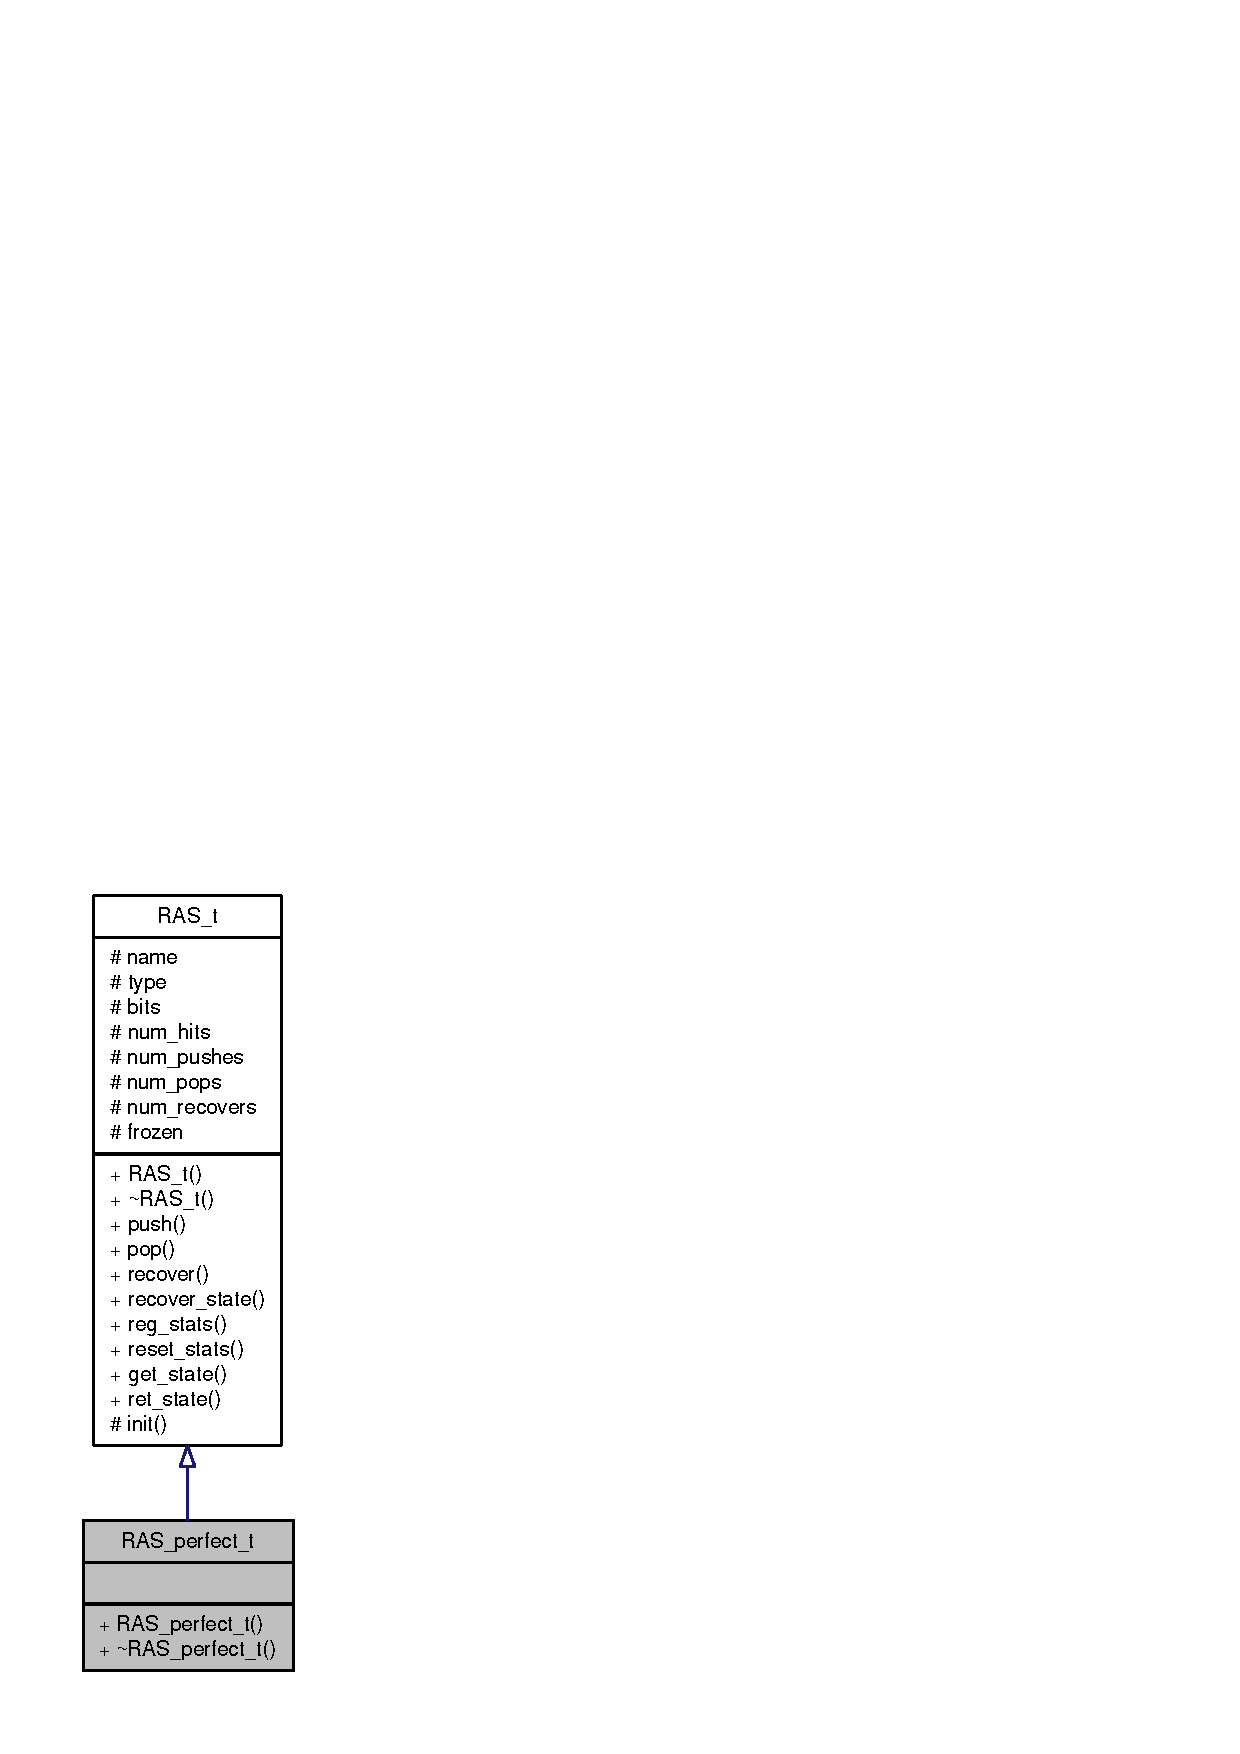
\includegraphics[height=400pt]{classRAS__perfect__t__inherit__graph}
\end{center}
\end{figure}
Collaboration diagram for RAS\_\-perfect\_\-t:\nopagebreak
\begin{figure}[H]
\begin{center}
\leavevmode
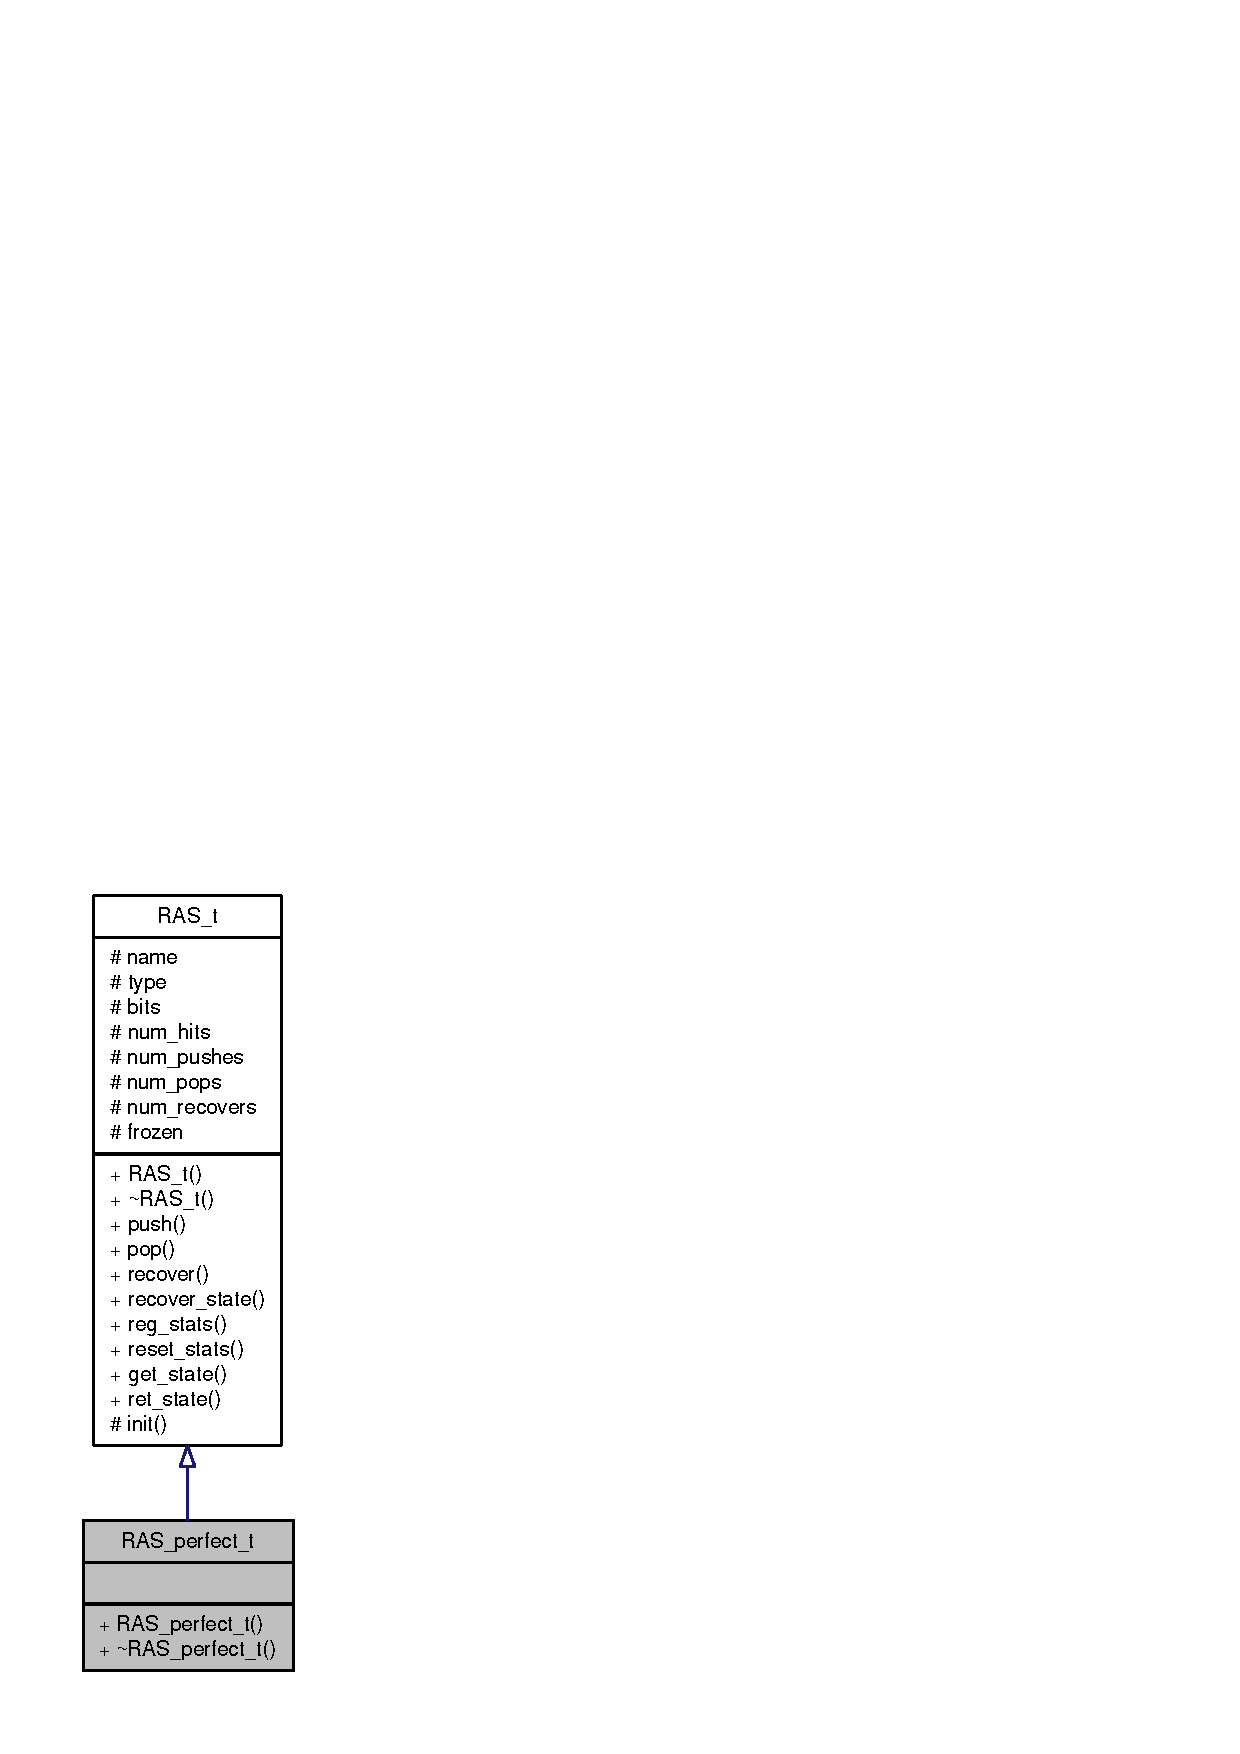
\includegraphics[height=400pt]{classRAS__perfect__t__coll__graph}
\end{center}
\end{figure}
\subsection*{Public Member Functions}
\begin{CompactItemize}
\item 
{\bf RAS\_\-perfect\_\-t} (void)
\item 
{\bf $\sim$RAS\_\-perfect\_\-t} ()
\end{CompactItemize}


\subsection{Detailed Description}


Definition at line 15 of file ras-perfect.cpp.

\subsection{Constructor \& Destructor Documentation}
\index{RAS\_\-perfect\_\-t@{RAS\_\-perfect\_\-t}!RAS\_\-perfect\_\-t@{RAS\_\-perfect\_\-t}}
\index{RAS\_\-perfect\_\-t@{RAS\_\-perfect\_\-t}!RAS_perfect_t@{RAS\_\-perfect\_\-t}}
\subsubsection[{RAS\_\-perfect\_\-t}]{\setlength{\rightskip}{0pt plus 5cm}RAS\_\-perfect\_\-t::RAS\_\-perfect\_\-t (void)\hspace{0.3cm}{\tt  [inline]}}\label{classRAS__perfect__t_dc20dc62084ec1021cb8319011f40581}




Definition at line 19 of file ras-perfect.cpp.

References COMPONENT\_\-NAME, fatal(), RAS\_\-t::init(), RAS\_\-t::name, and RAS\_\-t::type.\index{RAS\_\-perfect\_\-t@{RAS\_\-perfect\_\-t}!$\sim$RAS\_\-perfect\_\-t@{$\sim$RAS\_\-perfect\_\-t}}
\index{$\sim$RAS\_\-perfect\_\-t@{$\sim$RAS\_\-perfect\_\-t}!RAS_perfect_t@{RAS\_\-perfect\_\-t}}
\subsubsection[{$\sim$RAS\_\-perfect\_\-t}]{\setlength{\rightskip}{0pt plus 5cm}RAS\_\-perfect\_\-t::$\sim$RAS\_\-perfect\_\-t ()\hspace{0.3cm}{\tt  [inline]}}\label{classRAS__perfect__t_bc738f1b9afb8d49683a15c2bc1c0f64}




Definition at line 33 of file ras-perfect.cpp.

References RAS\_\-t::name, and RAS\_\-t::type.

The documentation for this class was generated from the following file:\begin{CompactItemize}
\item 
{\bf ras-perfect.cpp}\end{CompactItemize}
